% =============================================================================
% overview
% =============================================================================

To set the stage for what follows in this chapter, we first give a brief overview of some of the concepts in the \ER notation with the help of an example shown in \fig{eg1}. This example will be re-used throughout the description of the graphical symbols (glyphs) used by \SBGNERLone (with a few additions when the concepts are missing in the example) 

\begin{figure}[H]
  \centering
  \vspace*{-0.75em}
  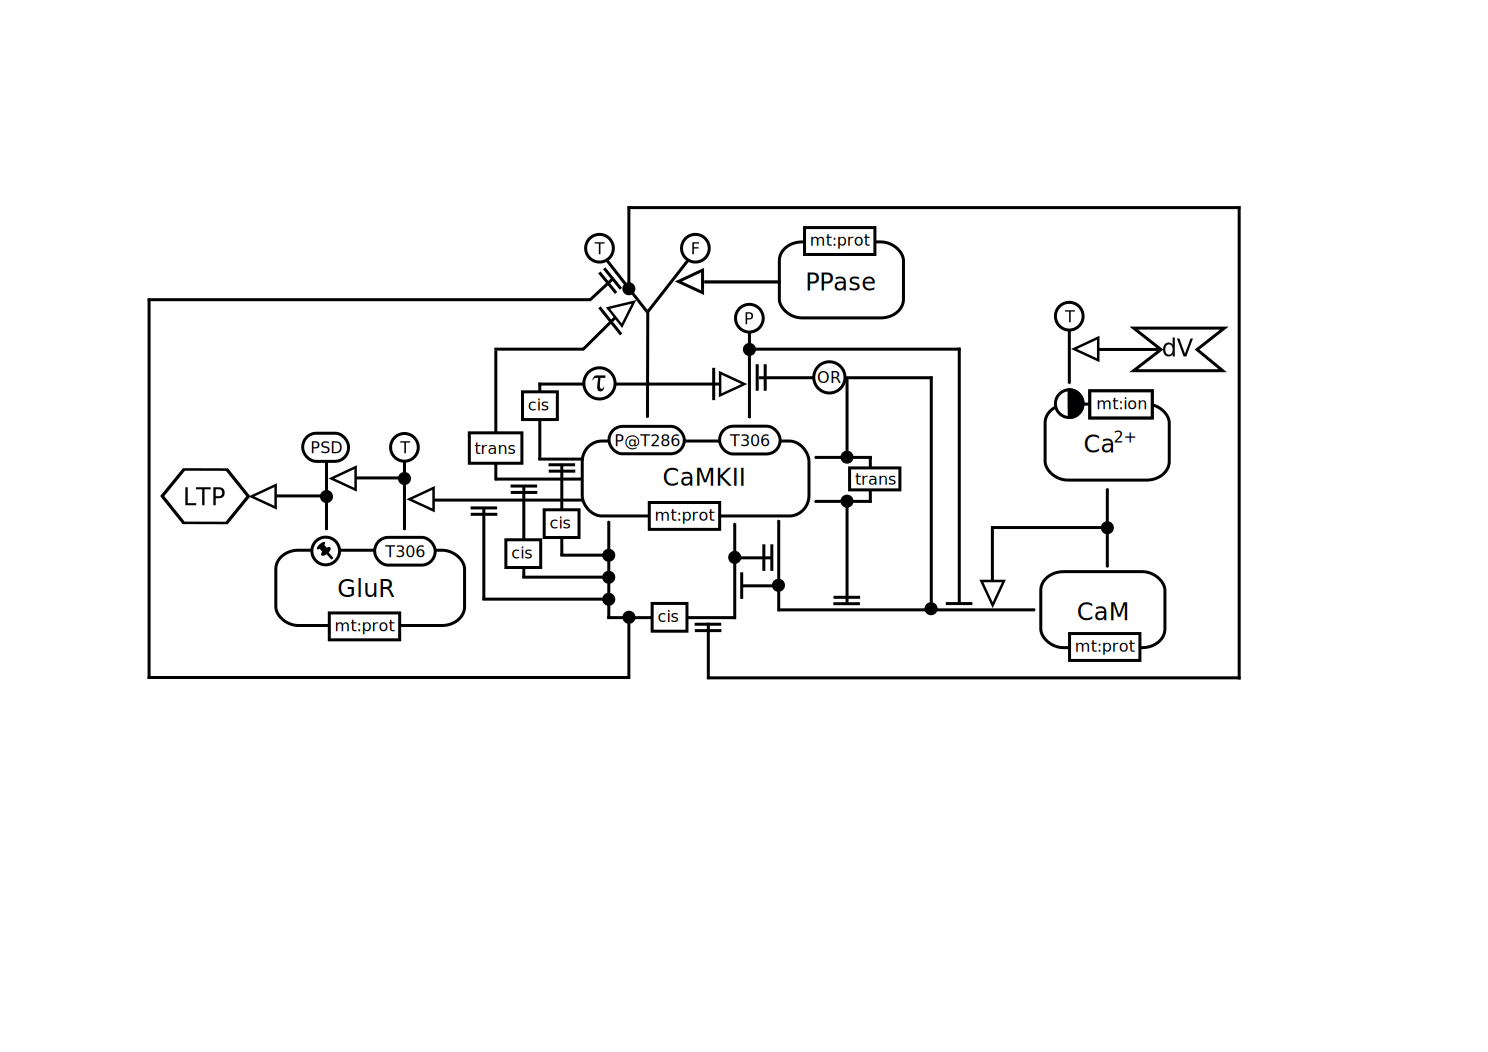
\includegraphics[scale=0.45]{examples/CaMKII-intro-new}
   \caption{This example of a \ER diagram depicts the effect of a depolarisation (dV) on the intracellular calcium, that binds to Calmodulin, that itself binds to the calcium/calmoduline kinase II (CaMKII). The binding of calmodulin inhibits the folding of CaMKII monomer on itself, thus relieving the inhibition on the kinase activity. The phosphorylation of the glutamate receptors finally leads to the Long Term Potentiation (LTP) of the synapses. In addition, the diagram shows the effect of trans-phosphorylation on threonine 286, that makes the enzyme constitutively active, and on threonine 306, that renders the kinase insensitive to calmodulin, as well as the dimerisation of the kinase.}
  \label{fig:eg1}
\end{figure}
 
The essence of the \ER diagram is to depict the influences of entities upon the behaviour of others. The entities are things that exist, either on their own or when statements become true. For instance, an entity can exist, different entities can interact, or a value can be assigned to an entity's property. The influences can therefore be understood as logical consequences of this existence. Contrary to the Process Diagram notation, where the different processes affect each other, the relationships are independent. On can imagine that each of the relationships represent a specific conclusion of a scientific experience or article. Their addition on a map represents the knowledge we have of the effects of the entities represented upon each other. The independence of relationships is the key to avoid the combinatorial explosion inherent to Process Diagrams.

\tab{component-summary} summarizes the different SBGN abstractions described in this chapter.
 
\newcolumntype{P}[1]{>{\raggedright\hspace{0pt}\arraybackslash}p{#1}}
 
 \begin{table}[h]
   \centering
   \small
   \begin{tabular}{@{}lP{2.4in}P{2.4in}@{}}
     \toprule
     \textbf{Component} & \textbf{Role} & \textbf{Examples}\\
     \midrule
     Entity node
     & Something that exists
     & An entity, the result of an interaction \\[0.5em]
 
     Statement	
     & Something that can be true or false
     & An interaction between entities, the assignment of a value to a variable \\[0.5em]
 
     Influence
     & The effect of something true on the realisation of a statement or another influence.
     & A stimulation, an absolute inhibition \\
     \bottomrule
   \end{tabular}
   \caption{Summary of \ER components and their roles.}
   \label{tab:component-summary}
 \end{table}

